\section{ Vaaratilanteet koneessa ja uloshypyssä }
\label{mahdolliset-vaaratilanteet-vaaratilanteet-koneessa-ja-uloshypyssa}

\subsection{ Repun aukeaminen koneessa }
\label{mahdolliset-vaaratilanteet-repun-aukeaminen-koneessa}


Repun (pää- tai varavarjon) tahaton aukeaminen johtuu yleensä hyppääjän varomattomasta liikkumisesta. Reppu, varavarjon kahva tai päävarjon aukaisujärjestelmä voivat tarttua jonnekin kiinni. Rauhallinen, tarpeettomia liikkeitä välttävä liikkuminen ehkäisee tarttumistilanteita tehokkaasti. Jos oma tai jonkun muun reppu kuitenkin aukeaa, estetään varjon avautuminen sekä ilmoitetaan asiasta hyppymestarille. 


Koneen lentäessä ovi auki on mahdollista, että reppu aukeaa ja varjo joutuu ilmavirtaan. Jos varjo purkautuu koneen sisällä ja ilmavirta tarttuu siihen, varjo voi vetää hyppääjän ulos. Tällaisessa tilanteessa sekä lentokone että hyppääjä voivat vahingoittua.  


Jos reppusi aukeaa ovella ja varjo karkaa ovesta ulos, hyppää ulos asennosta välittämättä. Tällaisessa tapauksessa hyppymestari auttaa sinut ripeästi ulos. Nopealla toiminnalla tilanne voidaan pelastaa. 

\subsection{ Hätähyppy }
\label{mahdolliset-vaaratilanteet-hatahyppy}


Jos lentäjän täytyy keventää konetta tai kone on ohjauskyvytön, hyppymestari antaa hyppääjille komennon HÄTÄHYPPY!  Komennolla OVELLE! siirrytään etuilematta ovelle ja komennolla MENE! poistutaan välittömästi. Hätähyppyä jatketaan, kunnes kaikki ovat hypänneet tai hyppymestari komentaa SEIS, PAKKOLASKU! Tällöin loput koneessa olevat valmistautuvat pakkolaskuun. 

\subsection{ Pakkolasku }
\label{mahdolliset-vaaratilanteet-pakkolasku}


Hyppytoiminnassa lennetään yleensä niin lähellä kenttää, että hyppykone pystyy liitämään takaisin esimerkiksi moottorihäiriön sattuessa. Tällöin hyppymestari ilmoittaa asiasta komennolla PAKKOLASKU! Automaattilaukaisin käännetään tällöin OFF-asentoon ja toimitaan ohjeiden mukaan. 


Kun kone on maassa ja pysähtynyt, on tulipalovaaran takia poistuttava nopeasti. Loukkaantuneita autetaan mahdollisuuksien mukaan. Hätähypyssä ja pakkolaskussa on muistettava, että lentäjä on koneen päällikkö mutta hyppääjien johtaja on hyppymestari. Oppilaille ohjeet tulevat \textbf{aina} hyppymestarilta. Tärkeintä on toimia rauhallisesti käskyjen mukaan. 

\subsection{ Koneeseen kiinni jääminen }
\label{mahdolliset-vaaratilanteet-koneeseen-kiinni-jaaminen}


Jos jäät roikkumaan koneeseen päävarjostasi, huomaat sen siitä, että roikut olkalukoista päävarjon kantohihnojen välityksellä. Yritä ottaa taivutettu asento jotta et pyöri ja voit varmistaa mistä olet kiinni. Varmistu, että olet hinauksessa vain olkalukkojen välityksellä jonka jälkeen tee varavarjotoimenpiteet. (\ref{paavarjon-vajaatoiminnot-varavarjon-kaytto} s.\pageref{paavarjon-vajaatoiminnot-varavarjon-kaytto}) 

\section{ Sotkeutuminen punoksiin }
\label{mahdolliset-vaaratilanteet-sotkeutuminen-punoksiin}


Jos uloshyppysi tai avausasentosi on huono, on mahdollista, että sotkeudut punoksiin. Pyri tällöin irrottautumaan takertuneista punoksista ennen varavarjotoimenpiteitä. Käytä tarvittaessa koukkupuukkoa. Tee kuitenkin varavarjotoimenpiteet (\ref{paavarjon-vajaatoiminnot-varavarjon-kaytto} s.\pageref{paavarjon-vajaatoiminnot-varavarjon-kaytto}) viimeistään 600 metrin korkeudessa. Punoksiin sotkeutumisen voi välttää keskittymällä hyvään asentoon ulos hypätessä ja varjoa avatessa. 

\section{ Apuvarjon aiheuttamat vaaratilanteet }
\label{mahdolliset-vaaratilanteet-apuvarjon-aiheuttamat-vaaratilanteet}


Huono avausasento voi johtaa siihen, että apuvarjon yhdyspunos kietoutuu esimerkiksi kätesi ympärille. Ravista kättäsi saadaksesi yhdyspunoksen irti. Jos et saa yhdyspunosta yhdellä yrityksellä irti tai et tiedä mihin se on tarttunut, tee varavarjotoimenpiteet. (\ref{paavarjon-vajaatoiminnot-varavarjon-kaytto} s.\pageref{paavarjon-vajaatoiminnot-varavarjon-kaytto}) Jos yhdyspunos on tarttunut käteesi, voit joutua tekemään varavarjotoimenpiteet yhdellä kädellä. Hyvällä uloshypyllä, avausasennolla sekä apuvarjon kunnollisella heittämisellä vapaaseen ilmavirtaan ehkäiset tehokkaasti edellisen kaltaisia vaaratilanteita. 


Apuvarjo voi avautumistilanteessa joskus tulla kuvun etureunan kautta kuvun alapuolelle. Tee ohjauskokeiluja saadaksesi selville käyttäytyykö varjo normaalisti. Jos varjo ei ohjaudu tai tekee rajuja liikkeitä, tee varavarjotoimenpiteet. (\ref{paavarjon-vajaatoiminnot-varavarjon-kaytto} s.\pageref{paavarjon-vajaatoiminnot-varavarjon-kaytto}) 


Avauksessa apuvarjo voi jäädä hyppääjän selän taakse muodostuvaan pyörteeseen eli turbulenssiin. Jos apuvarjon heiton jälkeen laskettuasi 105:een ei ole tapahtunut mitään, vilkaise olkapään yli (tarkasta). Asento kallistuu ja apuvarjon pitäisi saada ilmaa. Ellei varjo heti avaudu, tee varavarjotoimenpiteet, (\ref{paavarjon-vajaatoiminnot-varavarjon-kaytto} s.\pageref{paavarjon-vajaatoiminnot-varavarjon-kaytto}) koska apuvarjo tai yhdyspunos on saattanut tarttua johonkin kiinni tai reppu on jumissa. Kiinni tarttunutta osaa voidaan yrittää irrottaa, jos varmuudella nähdään ongelman aiheuttaja. Jos irrotus ei onnistu yhdellä yrityksellä tai et näe ongelman aiheuttajaa, tee varavarjotoimenpiteet heti. 

\section{ Vaaratilanteet varjon varassa }
\label{mahdolliset-vaaratilanteet-vaaratilanteet-varjon-varassa}

\subsection{ Kaksi varjoa auki }
\label{mahdolliset-vaaratilanteet-kaksi-varjoa-auki}


Yleisimmät syyt oppilailla kahden varjon varaan joutumisessa ovat matala avaus (itseaukaisuhypyillä), automaattilaukaisimen toimintahäiriö tai liian raju varjon käsittely (mm. poraaminen tai sakkaaminen). Kahden varjon tilanteissa ei lennetä laskeutumiskuviota. Mikäli toisen varjon puolijarrut ovat auki, pidä varjojen nopeus samana sopivilla jarruasetuksilla. 

%% Kahden liitovarjon yhdistelmä voi asettua erilaisiin muodostelmiin, jos molemmat varjot lentävät: 

\subsubsection{ Varjot peräkkäin (biplane) }
\label{mahdolliset-vaaratilanteet-varjot-perakkain-biplane}


Ohjaa varovasti etummaista varjoa vain välttämättömillä ohjausliikkeillä takimmaisista kantohihnoista. Älä avaa puolijarruja. Älä jarruta alastulossa ja valmistaudu kovaan alastuloon. 


\textbf{Älä päästä päävarjoa irti!} 


\begin{Figure}\centering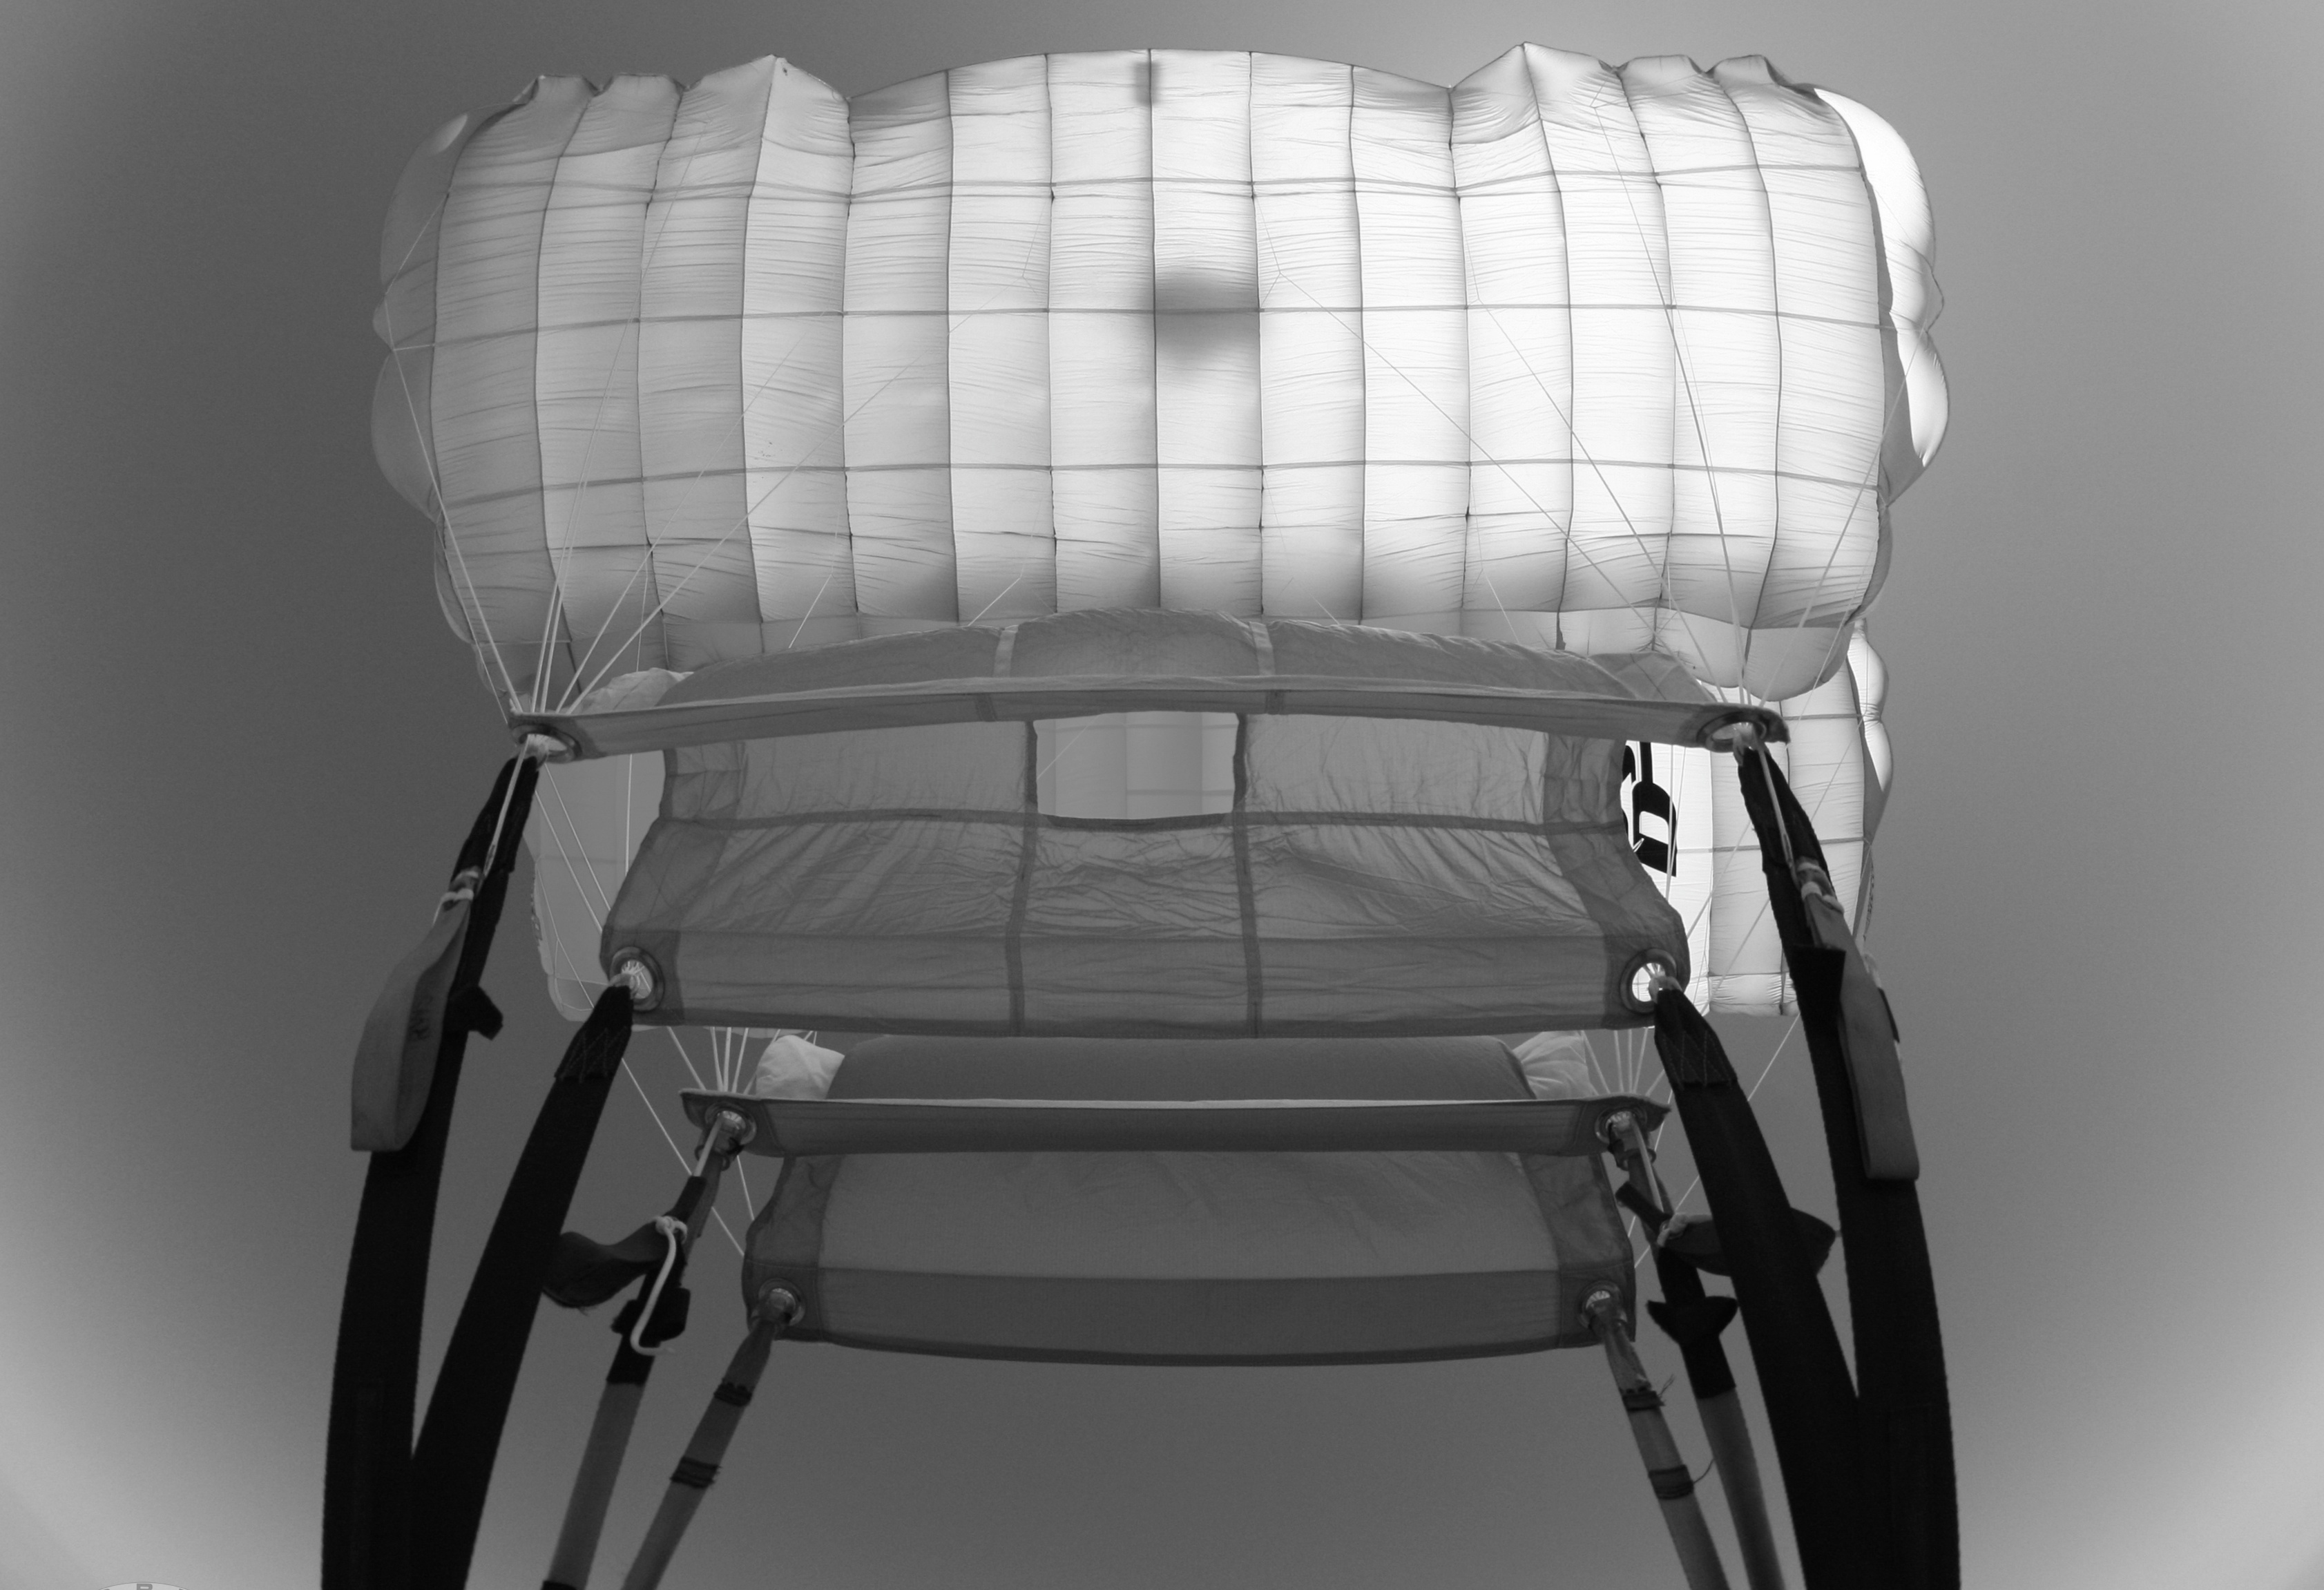
\includegraphics[width=0.95\textwidth]{2-kupua-biplane.jpeg}\captionof{figure}{Varjot peräkkäin (biplane)}\end{Figure} 

\subsubsection{ Varjot vierekkäin (side-by-side) }
\label{mahdolliset-vaaratilanteet-varjot-vierekkain-side-by-side}


Ohjaa varovasti hallitsevaa varjoa vain välttämättömillä ohjausliikkeillä takimmaisista kantohihnoista. Älä avaa puolijarruja. Älä jarruta alastulossa ja valmistaudu kovaan alastuloon. 


\textbf{Älä päästä päävarjoa irti!}  


\begin{Figure}\centering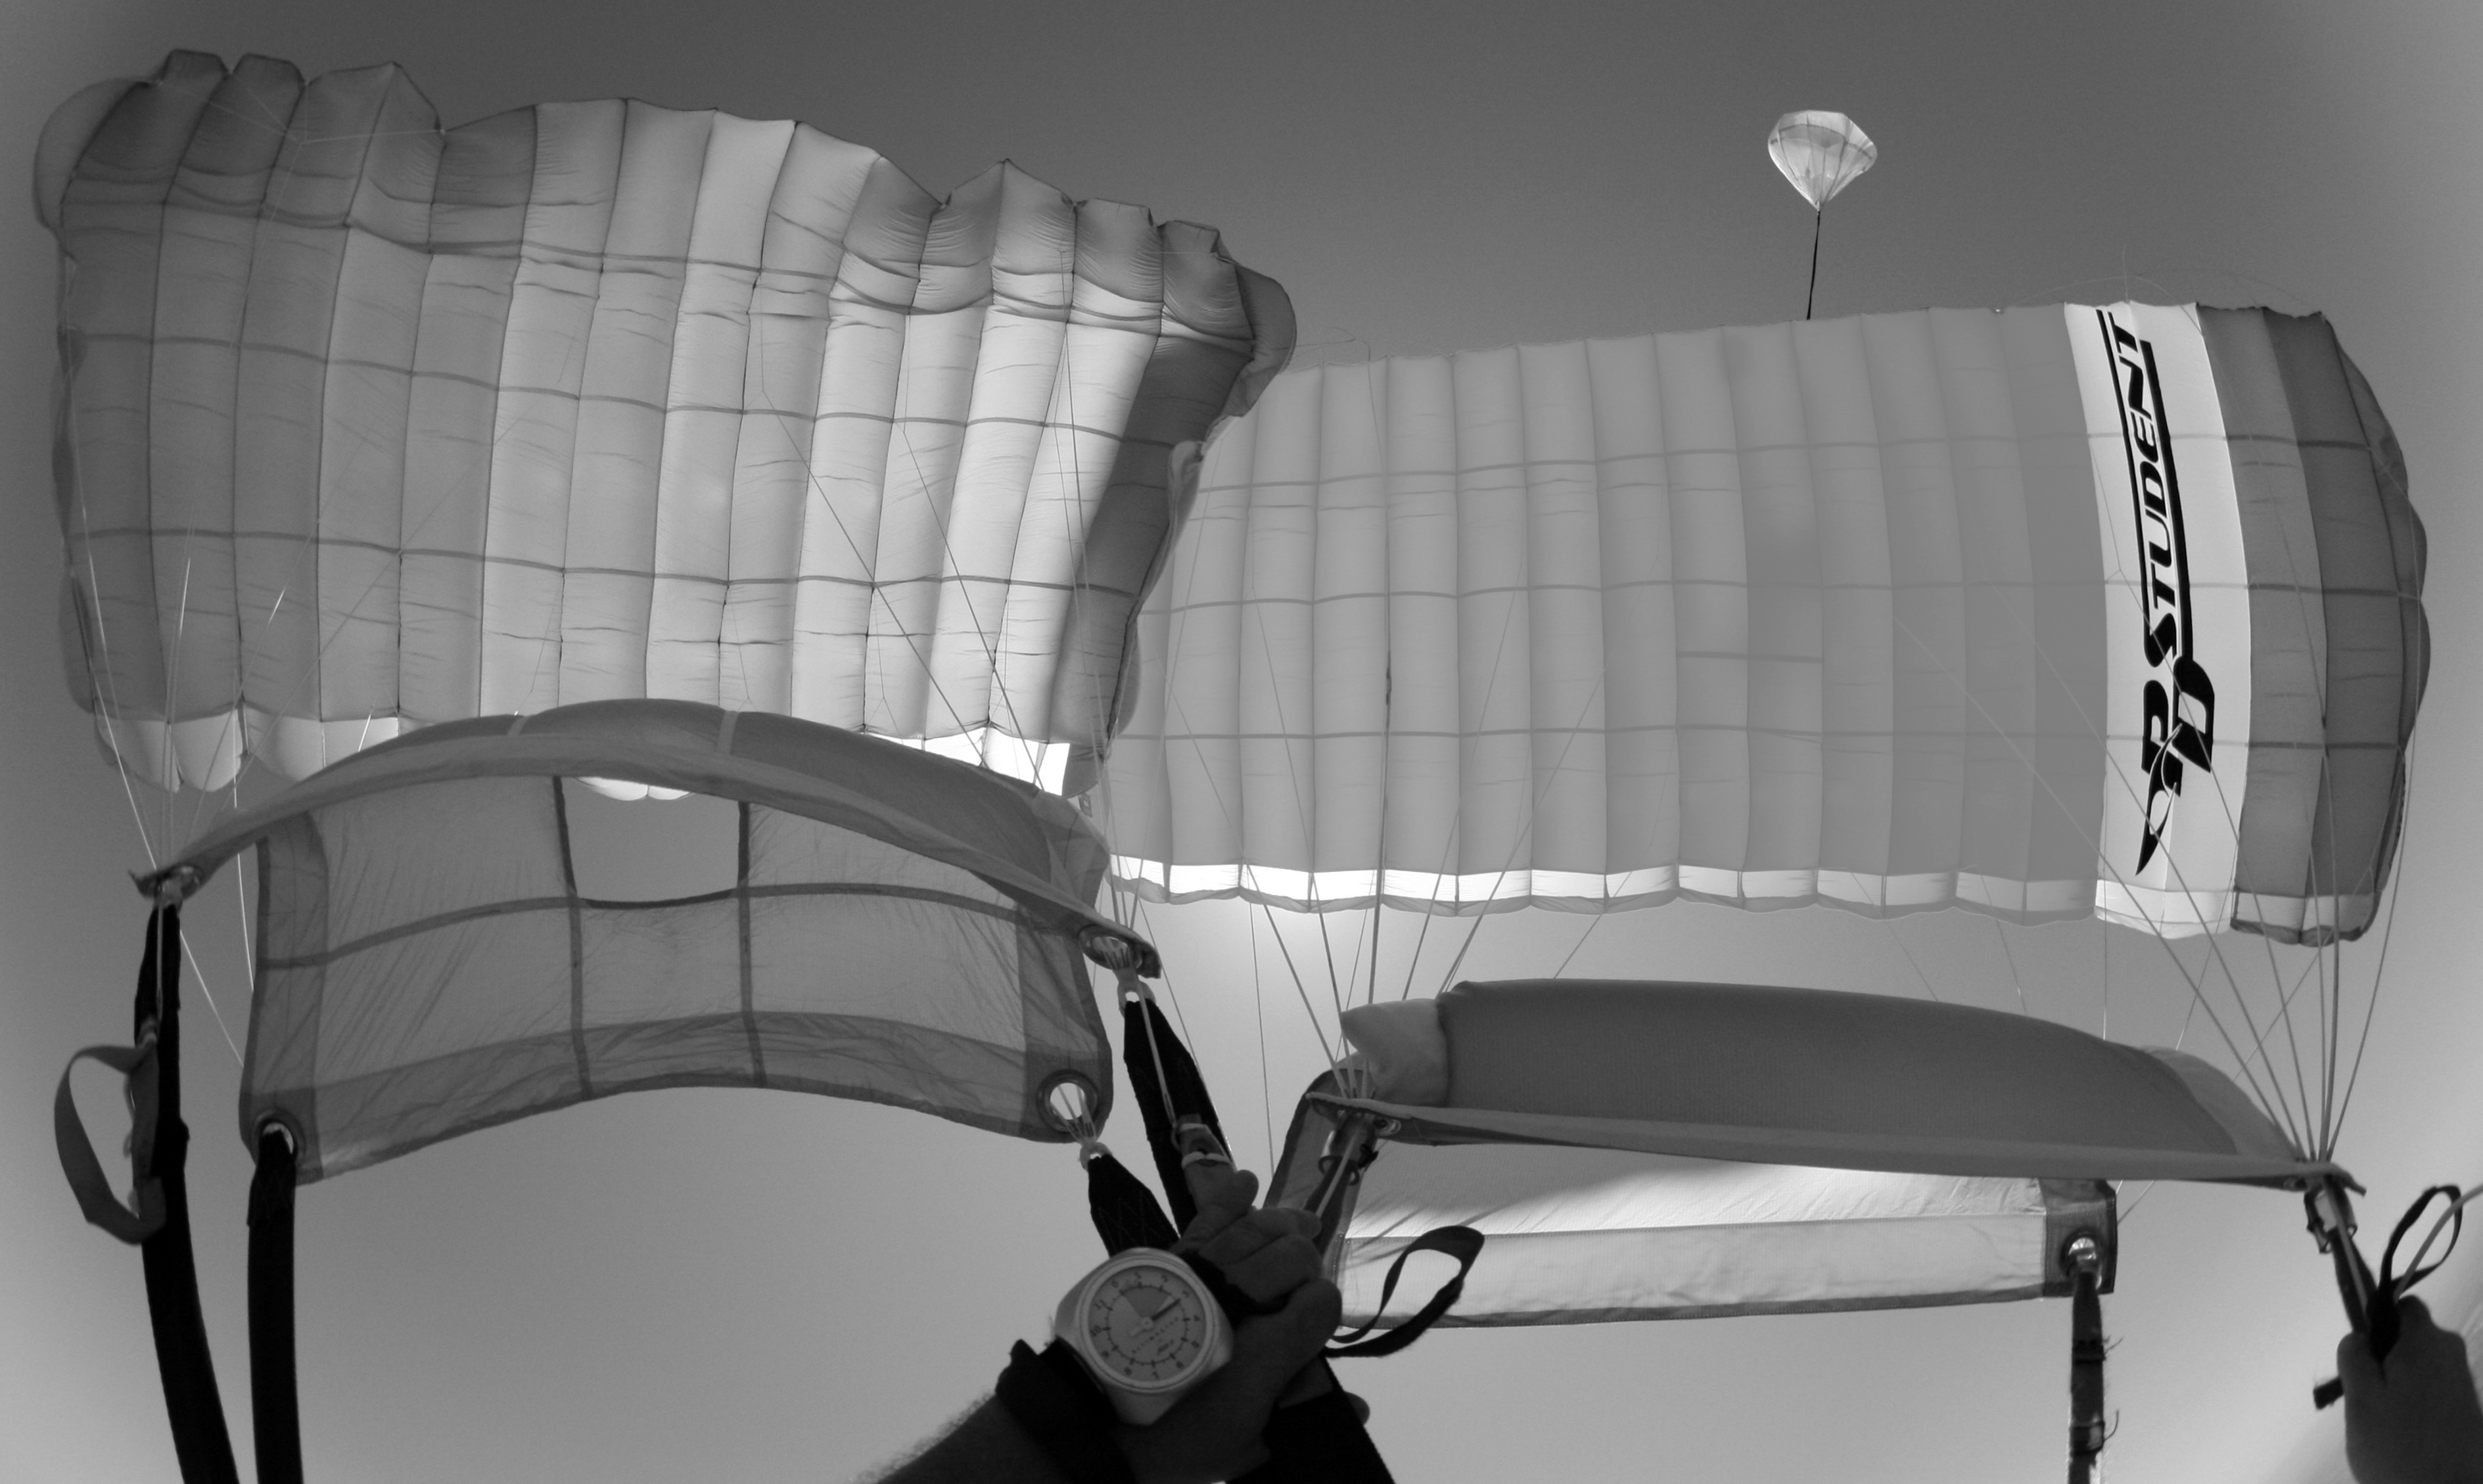
\includegraphics[width=0.95\textwidth]{2-kupua-sidebyside.jpeg}\captionof{figure}{Varjot vierekkäin (side-by-side)}\end{Figure} 

\subsubsection{ Varjot sivuilla, vajoavat nopeasti (downplane) }
\label{mahdolliset-vaaratilanteet-varjot-sivuilla-vajoavat-nopeasti-downplane}


Tämä lentotila on harvinainen. Varjot voivat siirtyä itsestään varjot vierekkäin -muodostelmaan. 


\textbf{Päästä päävarjo irti!} 


\begin{Figure}\centering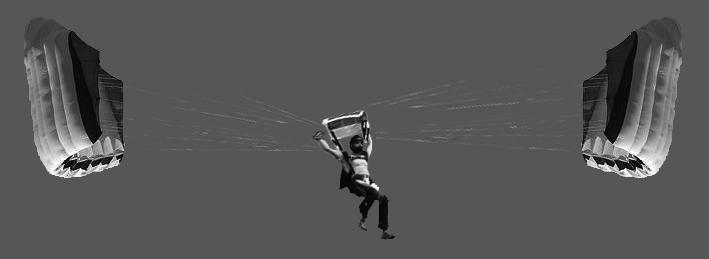
\includegraphics[width=0.95\textwidth]{2-kupua-downplane.jpeg}\captionof{figure}{Varjot sivuilla (downplane)}\end{Figure} 

\subsection{ Törmääminen varjon varassa }
\label{mahdolliset-vaaratilanteet-tormaaminen-varjon-varassa}


Törmäys on mahdollinen aina, kun ilmassa on useita hyppääjiä. Heti, kun olet tarkastanut, että varjo lentää, tarkasta ilmatila ja ole valmiina väistämään. Ennen puolijarrujen avaamista voit ohjata varjoa takimmaisista kantohihnoista (mikäli punokset eivät ole kierteellä). Väistä \textbf{oikealle!} 


Katso aina ennen käännöstä käännöksen suuntaan varmistaaksesi vapaa ilmatila. Alempana olevalla on aina etuajo-oikeus. Jos et voi välttää törmäämistä, minimoi törmäysvauhti jarruttamalla voimakkaasti sekä käperry \textit{palloksi.} Varoita toista hyppääjää huutamalla. 


Sotkeutumistilanteessa: 

\begin{itemize}
\item  Tarkkaile korkeutta, sillä päätökset on tehtävä riittävän korkealla 
\item  Keskustele aina kaverisi kanssa siitä, mitä aiotte tehdä 
\item  Varmista, että olet irti punoksista/kuvusta (käytä tarvittaessa koukkupuukkoa) ennen varavarjotoimenpiteitä. 
\end{itemize}

Jos ylempi varjo lentää ja alempi on sotkeutunut, voi alempi hyppääjä tehdä varavarjotoimenpiteet ja ylempi yleensä laskeutua päävarjollaan. Jos varjot ovat sotkeutuneet toisiinsa, joutuvat luultavasti molemmat tekemään varavarjotoimenpiteet. Tällöin molempien pitää sopia, missä järjestyksessä toimitaan, jotta vältetään törmääminen varavarjojen varassa. Jos korkeutta on liian vähän varavarjotoimenpiteisiin (alle 300 m), voi kaksikin ihmistä laskeutua yhdellä varjolla. 


Huomioi kaikissa toimenpiteissäsi ajan ja korkeuden menetys. 

\section{ Laskeutuminen epätavallisiin paikkoihin  }
\label{mahdolliset-vaaratilanteet-laskeutuminen-epatavallisiin-paikkoihin}


Laskeutumisen muihin paikkoihin kuin maalialueelle voi yleensä välttää ohjaamalla oikein. Alussa korkeuden ja kuljettavan matkan arviointi voi olla hankalaa, mutta hyppykokemuksen karttuessa tämäkin taito kehittyy. Joskus uloshyppypaikka voi olla väärä. Näin voi käydä etenkin, jos tuulet ovat yllättäen muuttuneet. Oli syy väärään uloshyppypaikkaan mikä tahansa, ajoissa tehty varalaskusuunnitelma mahdollistaa turvallisen laskeutumisen myös maalialueen ulkopuolelle. Suunnitelman muuttaminen viime hetkellä on vaarallista! 


Hyviä varalaskupaikkoja ovat esimerkiksi pellot ja muut aukeat alueet. Riippumatta siitä, mihin laskeudut, pyri aina laskeutumaan vastatuuleen! Pääasia on kuitenkin, että et tee jyrkkiä käännöksiä matalalla. Muista aina ottaa hyvä alastuloasento ja pitää se tiukasti maahan asti. 


Maalialueen ulkopuolelle laskeutuessasi et välttämättä enää loppuvaiheessa näe tuulipussia. Paina siksi mieleesi jo hypylle lähtiessäsi esimerkiksi se, missä suunnassa aurinko on, kun olet kääntynyt vastatuuleen. Liput, viirit ja savut ovat myös hyviä tuulen suunnan osoittimia. 

\subsection{ Laskeutuminen veteen }
\label{mahdolliset-vaaratilanteet-laskeutuminen-veteen}


Laskeudu mieluummin metsään kuin veteen. Joutuessasi laskeutumaan veteen pyri niin lähelle rantaa kuin mahdollista. Veteen laskeutuessasi toimi seuraavasti: 

\begin{itemize}
\item  Vapauta varavarjon pakkolaukaisuhihna 
\item  Käännä FXC OFF-asentoon 
\item  Löysää rintahihna 
\item  Ota alastuloasento 
\item  Tee loppuveto ennen veteen tuloa. 
\end{itemize}

Vedessä: 

\begin{itemize}
\item  Tukahduta varjo tarvittaessa tekemällä päävarjon irtipäästö 
\item  Avaa hihnat ja ui eroon varjosta. 
\end{itemize}
\subsection{ Laskeutuminen puuhun/metsään }
\label{mahdolliset-vaaratilanteet-laskeutuminen-puuhun-metsaan}


Puuhun tai metsään laskeutuessasi toimi seuraavasti: 

\begin{itemize}
\item  Vältä yksittäisiä ja korkeita puita 
\item  Ota alastuloasento ja vedä polvet ylös suojaamaan alavartaloa 
\item  Tee loppuveto puiden latvoihin sekä pidä kyynärpäät kyljissä kiinni 
\item  Valmistaudu tulemaan maahan asti ja pura alastuloasento vasta, kun liike loppuu. 
\end{itemize}

Jos jäät puuhun roikkumaan, älä pudottaudu korkealta, vaan odota apua. 


Suuri vaakanopeus aiheuttaa enemmän kolhuja kuin suuri vajoamisnopeus. Loppuvedon tekeminen puiden latvoihin on turvallisempaa kuin puita päin lentäminen. 

\subsection{ Laskeutuminen sähkölinjoihin }
\label{mahdolliset-vaaratilanteet-laskeutuminen-sahkolinjoihin}


Jos joudut laskeutumaan sähkölinjoihin, niin 

\begin{itemize}
\item  Heitä mahdollisesti käsissäsi olevat kahvat pois 
\item  Ohjaa varjoa loppuun saakka 
\item  Ota alastuloasento ja tee loppuveto linjoihin 
\item  Estä johtimien meno jalkojen väliin tai kainaloihin 
\item  Jos varjo jää kiinni, \textbf{älä yritä irrottaa sitä} 
\item  Odota apua. 
\end{itemize}
\subsection{ Laskeutuminen katolle }
\label{mahdolliset-vaaratilanteet-laskeutuminen-katolle}


Mikäli joudut laskeutumaan katolle, toimi seuraavasti: 

\begin{itemize}
\item  Ota alastuloasento 
\item  Tee loppuveto katolle 
\item  Tukahduta varjo välittömästi ja tee tarvittaessa päävarjon irtipäästö 
\item  Tartu kiinni kattorakenteista 
\item  Odota apua. 
\end{itemize}
\subsection{ Kiinteään esteeseen törmääminen }
\label{mahdolliset-vaaratilanteet-kiinteaan-esteeseen-tormaaminen}


Näitä ovat esimerkiksi seinät, autot, pylväät ja aidat. Jos osut kiinteään esteeseen, 

\begin{itemize}
\item  Tee loppuveto ennen törmäystä 
\item  Ota isku vastaan jaloilla 
\item  Valmistaudu maahantuloon 
\end{itemize}

Hyvän alastuloasennon merkitys korostuu, jos joudut laskeutumaan muualle kuin maalialueelle. 

